% Copyright 2026 Sreeram Anil
% SPDX-License-Identifier: CC-BY-4.0
% =============================================================================
%  Schmidt-Kalman ("consider") filter — robust_kalman family
% =============================================================================
\providecommand{\vf}{\bm{f}} \providecommand{\vh}{\bm{h}}
\providecommand{\vd}{\bm{d}} \providecommand{\mM}{\bm{M}}
\providecommand{\va}{\bm{a}} \providecommand{\vb}{\bm{b}}

\chapter{Schmidt--Kalman consider filter (Schmidt-KF)}
\label{ch:schmidtkf}

\section*{At a glance}
\begin{tabular}{@{}l>{\raggedright\arraybackslash}p{0.76\textwidth}@{}}
Family & Robust / embedded Kalman \\
Header & \texttt{include/estkit/filters/schmidt\_kf.hpp} \\
Registered name & \texttt{Schmidt-KF} \\
State dimension & $n_x = 4$ solve-for $+$ $n_c = 2$ consider states (generic in $n_x,n_c,n_u,n_y$) \\
Cost per step & $\mathcal{O}((n_x+n_c)^3)$; 1294\,ns/step, 8856\,B for the cell model, no heap \\
Primary references & \cite{schmidt1966,tapley2004,bucyjoseph1968,jazwinski1970} \\
\end{tabular}

\section{Motivation and aerospace/BMS relevance}
Every model-based state estimator is built on parameters that are themselves uncertain.  For the
equivalent-circuit cell model of Chapter~\ref{ch:ecm} the two dominant ones are the usable
capacity $Q$ and the series resistance $R_0$: the first drifts by tens of percent over the life of
the pack, the second grows with ageing and varies by more than a factor of two over the
automotive/aerospace temperature range.  The textbook remedy is \emph{joint} (augmented-state) or
\emph{dual} estimation --- add $\vtheta$ to the state vector and let the filter identify it.  That
only works when the mission excites the parameters persistently.  During an eVTOL flight the
current profile is dominated by two 75-second hover bursts and fifteen minutes of nearly constant
cruise; a joint filter asked to separate a capacity error from a resistance error from an SOC
error on this data is close to unidentifiable, and the usual failure mode is that the estimated
parameters absorb the SOC error and the filter quietly diverges.

Schmidt's \emph{consider} filter \cite{schmidt1966} takes the opposite --- and much more
conservative --- position.  The parameters are carried in the covariance but never corrected.
The filter is told ``$Q$ is known to $\pm5\,\%$ and $R_0$ to $\pm20\,\%$; account for that when
you decide how much to believe the voltmeter''.  It was invented for exactly this situation in
the Apollo navigation system, where the gravitational harmonics and station locations were
uncertain but hopelessly unobservable from the onboard measurements, and it remains the standard
tool of orbit determination \cite[Ch.~6]{tapley2004}.

For a BMS the pay-off is concrete and easy to see.  The terminal voltage is
$v = \ocv(\soc,T) + M h - v_1 - v_2 - R_0(T)\,i$.  At the 22.5\,A hover current of a
5\,Ah cell a $20\,\%$ uncertainty in $R_0$ is an uncertainty of 54\,mV in the
\emph{predicted} voltage --- twenty-five times the sensor noise.  An ordinary EKF does not know
this and reacts to the resulting residual as if it were an SOC error.  The consider filter
inflates the innovation covariance by exactly that amount and all but ignores the voltmeter while
the cell is being pulled hard, then trusts it again at low current.  It is automatic, requires no
extra states, and cannot be destabilised by a lack of excitation.

\section{Problem statement and assumptions}
The plant is the generic discrete-time model of the \code{estkit} model concept,
\begin{align}
\vx_{k+1} &= \vf(\vx_k,\vu_k;\vtheta) + \vw_k, & \vw_k &\sim \N{\bm 0}{\mQ_k}, \label{eq:sk-f}\\
\vy_k &= \vh(\vx_k,\vu_k;\vtheta) + \vv_k, & \vv_k &\sim \N{\bm 0}{\mR_k}, \label{eq:sk-h}
\end{align}
where $\vx_k\in\real^{n_x}$ is the \emph{solve-for} state, $\vu_k\in\real^{n_u}$ the input,
$\vy_k\in\real^{n_y}$ the measurement and
$\vtheta\in\real^{n_c}$ a vector of constant but uncertain model parameters, the
\emph{consider} parameters.  For the cell model $\vx=[\soc,v_1,v_2,h]^\T$, $\vu=[i,T]^\T$, $y=v$
and $\vtheta=[Q,R_0]^\T$, so $n_x=4$, $n_c=2$, $n_u=2$, $n_y=1$.

\begin{assumption}[Prior on the parameters]\label{as:sk-prior}
$\vtheta = \bar{\vtheta} + \delta\vtheta$ with $\bar{\vtheta}$ the nominal value supplied by the
BMS calibration and $\delta\vtheta\sim\N{\bm 0}{\mP_{cc,0}}$, independent of $\vx_0$, $\vw$, $\vv$.
$\mP_{cc,0}=\diag(\sigma_{c,1}^2,\dots,\sigma_{c,n_c}^2)$ is specified as a \emph{relative}
standard deviation, $\sigma_{c,j}=\rho_j\,|\bar{\theta}_j|$, because that is how parameter
tolerances are quoted on a data sheet.
\end{assumption}

\begin{assumption}[No correction of $\vtheta$]\label{as:sk-noupdate}
The estimate $\hat{\vtheta}_k \equiv \bar{\vtheta}$ for all $k$, and
$\mP_{cc,k}\equiv\mP_{cc,0}$: the parameter block of the gain is \emph{constrained to zero}.
\end{assumption}

Assumption~\ref{as:sk-noupdate} is what distinguishes the consider filter from joint estimation.
It is deliberately sub-optimal: the filter gives up the (possibly illusory) chance of learning
$\vtheta$ in exchange for a covariance that is guaranteed to remain conservative and a gain that
cannot be corrupted by an unidentifiable parameter direction.

\section{Derivation}

\subsection{Augmented system}
Stack the solve-for state and the parameters into
$\vx^a_k = \begin{bmatrix}\vx_k^\T & \vtheta^\T\end{bmatrix}^\T \in \real^{n_a}$,
$n_a = n_x+n_c$.  Since $\vtheta$ is constant,
\begin{equation}
\vx^a_{k+1} = \vf^a(\vx^a_k,\vu_k) + \begin{bmatrix}\vw_k\\ \bm 0\end{bmatrix},
\qquad
\vy_k = \vh^a(\vx^a_k,\vu_k) + \vv_k,
\label{eq:sk-aug}
\end{equation}
with $\vf^a = [\vf^\T\;\vtheta^\T]^\T$ and $\vh^a = \vh$.  Linearising about the current estimate
gives the partitioned Jacobians
\begin{equation}
\mF^a_k = \begin{bmatrix} \mF_k & \mF^{c}_k \\ \bm 0 & \mI_{n_c}\end{bmatrix}
   \in\real^{n_a\times n_a},
\qquad
\mH^a_k = \begin{bmatrix} \mH_k & \mH^{c}_k \end{bmatrix} \in\real^{n_y\times n_a},
\label{eq:sk-jac}
\end{equation}
where $\mF_k=\partial\vf/\partial\vx$, $\mH_k=\partial\vh/\partial\vx$ are the ordinary EKF
Jacobians and
\begin{equation}
\mF^{c}_k = \left.\frac{\partial \vf}{\partial\vtheta}\right|_{\hat{\vx}_k,\bar{\vtheta}}
\in\real^{n_x\times n_c},
\qquad
\mH^{c}_k = \left.\frac{\partial \vh}{\partial\vtheta}\right|_{\hat{\vx}_k,\bar{\vtheta}}
\in\real^{n_y\times n_c}
\label{eq:sk-sens}
\end{equation}
are the \emph{sensitivity} matrices: they say how a parameter error propagates into the state and
into the predicted measurement.  In \code{estkit} they are produced by
\code{AugmentedModel<Model>} from \code{core/model.hpp}, which obtains $\mF_k,\mH_k$ from the
model's analytic Jacobians and $\mF^c_k,\mH^c_k$ by central differences on
\code{Model::set\_params}, so no battery-specific code enters the filter.

Write the augmented covariance in blocks,
\begin{equation}
\mP^a_k = \begin{bmatrix} \mP_{xx,k} & \mP_{xc,k}\\ \mP_{xc,k}^\T & \mP_{cc,k}\end{bmatrix},
\qquad \mP_{xx}\in\real^{n_x\times n_x},\;\mP_{xc}\in\real^{n_x\times n_c},\;
\mP_{cc}\in\real^{n_c\times n_c}.
\label{eq:sk-blocks}
\end{equation}

\subsection{Time update}
Propagating $\mP^a$ through \eqref{eq:sk-jac} and adding
$\mQ^a=\diag(\mQ,\bm 0)$ gives, block by block,
\begin{align}
\mP^-_{xx} &= \mF\mP^+_{xx}\mF^\T + \mF\mP^+_{xc}(\mF^{c})^\T + \mF^{c}(\mP^+_{xc})^\T\mF^\T
              + \mF^{c}\mP_{cc}(\mF^{c})^\T + \mQ, \label{eq:sk-tuxx}\\
\mP^-_{xc} &= \mF\mP^+_{xc} + \mF^{c}\mP_{cc}, \label{eq:sk-tuxc}\\
\mP^-_{cc} &= \mP_{cc}. \label{eq:sk-tucc}
\end{align}
Equation~\eqref{eq:sk-tuxx} is the heart of a consider analysis: the term
$\mF^{c}\mP_{cc}(\mF^{c})^\T$ injects, at every step, the state uncertainty generated by the
parameter error.  For the cell model the only non-zero entry of $\mF^c$ is
$\partial \soc_{k+1}/\partial Q = \eta\,\dt\, i/(3600\,Q^2)$, so
\eqref{eq:sk-tuxx} makes the SOC variance grow quadratically in the accumulated
ampere-hours --- precisely the behaviour of a Coulomb counter with a capacity error, which the
standard EKF covariance does not model at all.

\subsection{Measurement update with a constrained gain}
Let $\veps_k = \vy_k - \vh(\xminus_k,\vu_k)$ be the innovation.  For the augmented system the
innovation covariance and the state/measurement cross-covariance are
\begin{align}
\mS_k &= \mH^a\mP^{a-}(\mH^a)^\T + \mR \nonumber\\
      &= \underbrace{\mH\mP^-_{xx}\mH^\T + \mR}_{\text{ordinary EKF}}
       + \underbrace{\mH\mP^-_{xc}(\mH^{c})^\T + \mH^{c}(\mP^-_{xc})^\T\mH^\T
        + \mH^{c}\mP_{cc}(\mH^{c})^\T}_{\text{consider contribution}}, \label{eq:sk-S}\\
\mP^-_{xy} &= \mP^-_{xx}\mH^\T + \mP^-_{xc}(\mH^{c})^\T, \qquad
\mP^-_{cy} = (\mP^-_{xc})^\T\mH^\T + \mP_{cc}(\mH^{c})^\T. \label{eq:sk-Pxy}
\end{align}
The optimal (Kalman) augmented gain would be
$\mK^a=[\mP^{-\T}_{xy}\;\mP^{-\T}_{cy}]^\T\mS^{-1}$.  Assumption~\ref{as:sk-noupdate} replaces it
by the \emph{consider gain}
\begin{equation}
\boxed{\;\mK^a_k = \begin{bmatrix}\mK_{x,k}\\ \bm 0\end{bmatrix},\qquad
\mK_{x,k} = \mP^-_{xy}\,\mS_k^{-1}\in\real^{n_x\times n_y}.\;}
\label{eq:sk-gain}
\end{equation}
The state update is $\xplus_k = \xminus_k + \mK_{x,k}\veps_k$ and $\hat{\vtheta}$ is untouched.

\begin{remark}[The Joseph form is mandatory]\label{rem:sk-joseph}
The familiar short covariance update $\mP^+=(\mI-\mK\mH)\mP^-$ is valid \emph{only} for the
optimal gain, because its derivation cancels a term proportional to
$\mK\mS - \mP^-\mH^\T$, which vanishes only when $\mK=\mP^-\mH^\T\mS^{-1}$.  The consider gain
\eqref{eq:sk-gain} is by construction sub-optimal for the augmented system, so the general
(Joseph) form \cite{bucyjoseph1968} must be used:
\begin{equation}
\mP^{a+}_k = (\mI_{n_a}-\mK^a_k\mH^a_k)\,\mP^{a-}_k\,(\mI_{n_a}-\mK^a_k\mH^a_k)^\T
            + \mK^a_k\mR_k(\mK^a_k)^\T .
\label{eq:sk-joseph}
\end{equation}
With $\mK^a=[\mK_x^\T\;\bm 0]^\T$ the bottom block row of $\mI-\mK^a\mH^a$ is
$[\bm 0\;\;\mI_{n_c}]$, so \eqref{eq:sk-joseph} automatically reproduces Schmidt's
partitioned recursion
\begin{align}
\mP^+_{xx} &= (\mI-\mK_x\mH)\mP^-_{xx}(\mI-\mK_x\mH)^\T
   - (\mI-\mK_x\mH)\mP^-_{xc}(\mH^c)^\T\mK_x^\T \nonumber\\
   &\qquad - \mK_x\mH^c(\mP^-_{xc})^\T(\mI-\mK_x\mH)^\T
   + \mK_x\!\left[\mH^c\mP_{cc}(\mH^c)^\T+\mR\right]\!\mK_x^\T, \label{eq:sk-pxx}\\
\mP^+_{xc} &= \mP^-_{xc} - \mK_x\!\left[\mH\mP^-_{xc} + \mH^c\mP_{cc}\right]
            = \mP^-_{xc} - \mK_x (\mP^-_{cy})^\T, \label{eq:sk-pxc}\\
\mP^+_{cc} &= \mP_{cc}. \label{eq:sk-pcc}
\end{align}
Equation~\eqref{eq:sk-pcc} is the defining property: \textbf{the consider covariance is never
reduced}, so the filter never becomes more confident about $\vtheta$ than its prior allows, no
matter how long the mission lasts.  The implementation evaluates \eqref{eq:sk-joseph} directly on
the $n_a\times n_a$ matrix, which is both shorter and numerically better conditioned than
\eqref{eq:sk-pxx}--\eqref{eq:sk-pcc}.
\end{remark}

\begin{proposition}[Consistency]\label{prop:sk-cons}
Under Assumption~\ref{as:sk-prior} and exact linearity, the recursion
\eqref{eq:sk-tuxx}--\eqref{eq:sk-pcc} yields
$\mP_{xx,k} = \E{(\vx_k-\xhat_k)(\vx_k-\xhat_k)^\T}$ exactly, i.e.\ the reported covariance is the
true error covariance of the (sub-optimal) estimator, including the contribution of the parameter
error.  By contrast an EKF that ignores $\delta\vtheta$ reports a covariance that is
\emph{smaller} than the true error covariance by
$\mA_k\mP_{cc}\mA_k^\T \succeq \bm 0$, where $\mA_k=\partial\xhat_k/\partial\vtheta$ is the
accumulated parameter sensitivity of the estimate.
\end{proposition}
\noindent The proof is the standard covariance-propagation argument through
\eqref{eq:sk-aug} with the gain restricted as in \eqref{eq:sk-gain}; see
\cite[\S6.5]{tapley2004}.  Proposition~\ref{prop:sk-cons} is why the method is called
\emph{consider covariance analysis}: it is the smallest modification of the Kalman filter that
restores consistency in the presence of unmodelled parameter error.

\section{Algorithm}
\begin{algorithm}[H]
\caption{Schmidt-KF --- one sampling period}
\begin{algorithmic}[1]
\Require $\xplus_{k-1},\;\mP^{a+}_{k-1},\;\bar{\vtheta},\;\vu_{k-1},\;\vy_k,\;\vu_k$
\State \textbf{Time update:}
  $\mF^a \gets \eqref{eq:sk-jac}$ at $(\hat{\vx}^a_{k-1},\vu_{k-1})$
\State $\hat{\vx}^a_k \gets \vf^a(\hat{\vx}^a_{k-1},\vu_{k-1})$ \Comment{$\vtheta$ block copied}
\State $\mP^{a-}_k \gets \mF^a\mP^{a+}_{k-1}(\mF^a)^\T + \diag(\mQ_k,\bm 0)$; symmetrise
\State \textbf{Measurement update:}
  $\mH^a \gets \eqref{eq:sk-jac}$ at $(\hat{\vx}^a_k,\vu_k)$; $\mR\gets\mR_k$
\State $\mP^{a-}_{y}\gets \mP^{a-}_k(\mH^a)^\T$ \Comment{stacked $[\mP_{xy};\mP_{cy}]$}
\State $\mS_k \gets \mH^a\mP^{a-}_{y} + \mR$ \Comment{consider-inflated, Eq.~\eqref{eq:sk-S}}
\State $\mK^a_k \gets \mP^{a-}_{y}\mS_k^{-1}$, then \textbf{zero its last $n_c$ rows}
       \Comment{Eq.~\eqref{eq:sk-gain}}
\State $\veps_k \gets \vy_k - \vh(\xminus_k,\vu_k)$;\quad
       $\hat{\vx}^a_k \gets \hat{\vx}^a_k + \mK^a_k\veps_k$
\State $\mP^{a+}_k \gets (\mI-\mK^a_k\mH^a)\mP^{a-}_k(\mI-\mK^a_k\mH^a)^\T+\mK^a_k\mR(\mK^a_k)^\T$
       \Comment{Joseph, Eq.~\eqref{eq:sk-joseph}}
\State symmetrise; apply \code{constrain} to the $\vx$ block
\Ensure $\xplus_k = [\mI_{n_x}\;\bm 0]\hat{\vx}^a_k$,\quad
        $\Pplus_k = [\mI_{n_x}\;\bm 0]\mP^{a+}_k[\mI_{n_x}\;\bm 0]^\T$
\end{algorithmic}
\end{algorithm}

\section{Application to the battery model}
With $\vtheta=[Q,R_0]^\T$ the sensitivities \eqref{eq:sk-sens} are, analytically,
\begin{equation}
\mF^{c} = \begin{bmatrix}
 \dfrac{\eta(i)\,\dt\, i}{3600\,Q^{2}} & 0\\[4pt] 0&0\\ 0&0\\
 \dfrac{\partial a_h}{\partial Q}\,(h+\sgn i) & 0
\end{bmatrix},
\qquad
\mH^{c} = \begin{bmatrix} 0 & -\,i\,\alpha_{R_0}(T)\end{bmatrix},
\label{eq:sk-batt}
\end{equation}
where $\alpha_{R_0}(T)=\exp\!\big[\tfrac{E_{a,R_0}}{R_g}(\tfrac1T-\tfrac1{T_{\mathrm{ref}}})\big]$
is the Arrhenius factor of Chapter~\ref{ch:ecm} (the implementation obtains both by central
differences, so these expressions are only used here for interpretation).

The dominant term is $\mH^c\mP_{cc}(\mH^c)^\T = i^2\alpha_{R_0}^2\sigma_{R_0}^2$ in
\eqref{eq:sk-S}.  With the registered defaults $\rho_Q = 5\,\%$ (cell-to-cell spread plus
ageing between re-calibrations) and $\rho_{R_0} = 20\,\%$ (Arrhenius scatter plus the
$\sim\!25\,\%$ resistance growth that accompanies a $10\,\%$ capacity fade in the plant's ageing
law), one obtains at 25\,\ensuremath{{}^\circ}C
\[
\sqrt{\mH^c\mP_{cc}(\mH^c)^\T} = 0.20\times12\,m\ensuremath{\Omega}\times i
  = \begin{cases} 13\,mV & i=5.5\,A\ (\text{cruise}),\\
                  54\,mV & i=22.5\,A\ (\text{hover}),\end{cases}
\]
against $\sqrt{\mR}=2.1\,mV$.  The innovation covariance is therefore inflated by a
factor of $\sim\!40$ in cruise and $\sim\!660$ in hover, and the gain is reduced accordingly.  In
the \texttt{cold} scenario the Arrhenius factor is $\alpha_{R_0}(263\,K)=2.09$ and the
inflation grows by another factor of four --- which, as the benchmark shows, is the one place
where the method costs accuracy.

\section{Implementation notes}
\begin{itemize}[nosep]
\item \textbf{Dimensions.}  The filter works on $n_a=6$ matrices instead of $n_x=4$, i.e.\
$\left(6/4\right)^3 = 3.4\times$ the flops of an EKF.  Measured: 1294\,ns/step
against 478\,ns for the EKF, a factor $2.7$ --- close to the cubic prediction, the remainder
being the numeric differentiation of $\mF^c,\mH^c$, which costs $2n_c$ extra evaluations of
$\vf$ and $\vh$ per step.
\item \textbf{Memory.}  8856\,B against the EKF's 4336\,B.  Only 520\,B of the difference is the
$6\times6$ augmented covariance, the augmented gain and the parameter block; the remaining
$\approx4$\,kB is a \emph{second copy of the model}.  \code{AugmentedModel} keeps one mutable
scratch instance of \code{Model} whose parameters are overwritten in place by \code{with()},
so that a call to $\vf$, $\vh$, $\mQ$ or $\mR$ at a perturbed $\vtheta$ does not have to copy
the whole model --- for the cell model that would mean copying the 3856\,B OCV table six times
per step.  The trade is 4\,kB of flash-resident-in-principle data against a factor of two in
runtime, and for a single-cell estimator it is clearly worth it; for a per-cell instance on a
100-cell pack one would hoist the OCV table out of the model first.
\item \textbf{Analytic sensitivities.}  Supplying $\mF^c,\mH^c$ analytically instead of by
finite differences would bring the cost down to about 700\,ns/step.  The generic
implementation deliberately does not, so that the filter works for any model exposing
\code{params()}/\code{set\_params()}.
\item \textbf{Joseph everywhere.}  As shown in Remark~\ref{rem:sk-joseph} the short form is
\emph{wrong} here, not merely less stable; the option to disable it has therefore been removed
from \code{Options}.
\item \textbf{$\mP_{cc}$ is structurally constant.}  \code{opts.q\_theta} allows a slow random
walk on $\vtheta$ (a ``consider filter with drifting parameters''); it defaults to zero, which is
the classical analysis.  Note that a non-zero \code{q\_theta} makes $\mP_{cc}$ \emph{grow}, never
shrink, because the gain block stays zero.
\item \textbf{Guards.}  $\mS^{-1}$ is checked with \code{is\_finite()} before use; if it fails the
prior is kept.  The augmented covariance is symmetrised after both updates.  No heap, no
exceptions, no dynamic dimensions.
\item \textbf{float32.}  The \code{-DESTKIT\_FLOAT=ON} build reproduces the double results to
two digits (\texttt{nominal} $0.39/0.51\,\%$ vs.\ $0.38/0.46\,\%$, \texttt{combined}
$5.06/1.16\,\%$ vs.\ $5.20/1.09\,\%$, \texttt{param\_mismatch} $0.44/0.37\,\%$ vs.\
$0.51/0.45\,\%$) and halves the footprint to 4428\,B; the $6\times6$ Joseph form is
well conditioned because $\mP_{cc}$ never shrinks towards singularity.
\item \textbf{Cortex-M7 estimate.}  $\sim\!2600$ flops/step for $n_a=6,n_y=1$ including the two
extra model evaluations; at 300\,MHz with a single-precision FPU this is
$\approx30\,\ensuremath{\mu}s$, i.e.\ $0.03\,\%$ duty at the 10\,Hz sample rate of this
benchmark, or $\approx3\,\%$ if run on 100 cells sequentially.
\item \textbf{Limitation.}  The filter never learns $\vtheta$; \code{capacity\_Ah()} is therefore
not provided.  If the mission does excite the parameters, a joint/dual filter will beat it.
\end{itemize}

\section{Benchmark results}
% Copyright 2026 Sreeram Anil
% SPDX-License-Identifier: CC-BY-4.0
\begin{table}[H]\centering\footnotesize\setlength{\tabcolsep}{4pt}
\caption{Schmidt-KF: cell-level benchmark on the eVTOL mission (mean over seeds; RMSE and max error in \% SOC; $t_\mathrm{conv}$: first time the error stays below 2\,\% for 60\,s, -- = never; EKF reference: steady-state RMSE of the plain EKF on the same data).}\label{tab:cell_SchmidtKF}
\begin{tabular}{llrrrrrcrr}\toprule
plant & scenario & RMSE & RMSE$_\mathrm{ss}$ & max & $t_\mathrm{conv}$ [s] & RMSE$_v$ [mV] & div. & EKF ref. & ns/step \\ \midrule
ECM & nominal & 0.38 & 0.46 & 1.04 & 0 & 3.84 & no & 0.05 & 1293 \\
ECM & init\_error & 0.43 & 0.46 & 0.85 & 0 & 4.56 & no & 0.05 & 1324 \\
ECM & current\_bias & 0.33 & 0.33 & 1.40 & 0 & 9.10 & no & 0.61 & 1301 \\
ECM & noise\_step & 0.87 & 1.14 & 3.47 & 0 & 7.24 & no & 0.12 & 1307 \\
ECM & outliers & 0.77 & 0.83 & 3.16 & 8 & 6.56 & no & 0.21 & 1297 \\
ECM & cold & 1.42 & 1.54 & 1.94 & 0 & 15.88 & no & 0.16 & 1300 \\
ECM & hot & 0.23 & 0.21 & 1.00 & 0 & 1.97 & no & 0.03 & 1302 \\
ECM & aged\_cell & 0.71 & 0.59 & 1.54 & 0 & 36.55 & no & 1.52 & 1296 \\
ECM & param\_mismatch & 0.51 & 0.45 & 1.19 & 0 & 18.18 & no & 1.36 & 1307 \\
ECM & sensor\_dropout & 0.38 & 0.46 & 1.04 & 0 & 3.83 & no & 0.46 & 1304 \\
ECM & preisach & 1.02 & 0.55 & 2.09 & 21 & 7.29 & no & 0.20 & 1306 \\
ECM & combined & 5.20 & 1.09 & 10.95 & 1038 & 28.17 & no & 12.44 & 1323 \\
\midrule
SPM & nominal & 0.69 & 0.51 & 1.59 & 0 & 7.49 & no & 3.73 & 1230 \\
SPM & init\_error & 1.31 & 0.60 & 2.64 & 360 & 8.25 & no & 3.81 & 1233 \\
SPM & current\_bias & 1.02 & 0.71 & 2.23 & 0 & 10.83 & no & 5.69 & 1232 \\
SPM & noise\_step & 1.08 & 1.26 & 5.20 & 0 & 9.36 & no & 3.30 & 1232 \\
SPM & outliers & 1.19 & 0.95 & 3.46 & 200 & 8.91 & no & 1.99 & 1230 \\
SPM & cold & 2.49 & 2.44 & 5.67 & 939 & 34.96 & no & 7.35 & 1198 \\
SPM & hot & 0.43 & 0.44 & 1.42 & 0 & 5.76 & no & 2.16 & 1232 \\
SPM & param\_mismatch & 1.10 & 0.75 & 2.66 & 0 & 14.21 & no & 3.13 & 1227 \\
SPM & sensor\_dropout & 0.69 & 0.50 & 1.58 & 0 & 7.48 & no & 5.31 & 1230 \\
\bottomrule\end{tabular}\end{table}

\begin{figure}[H]\centering
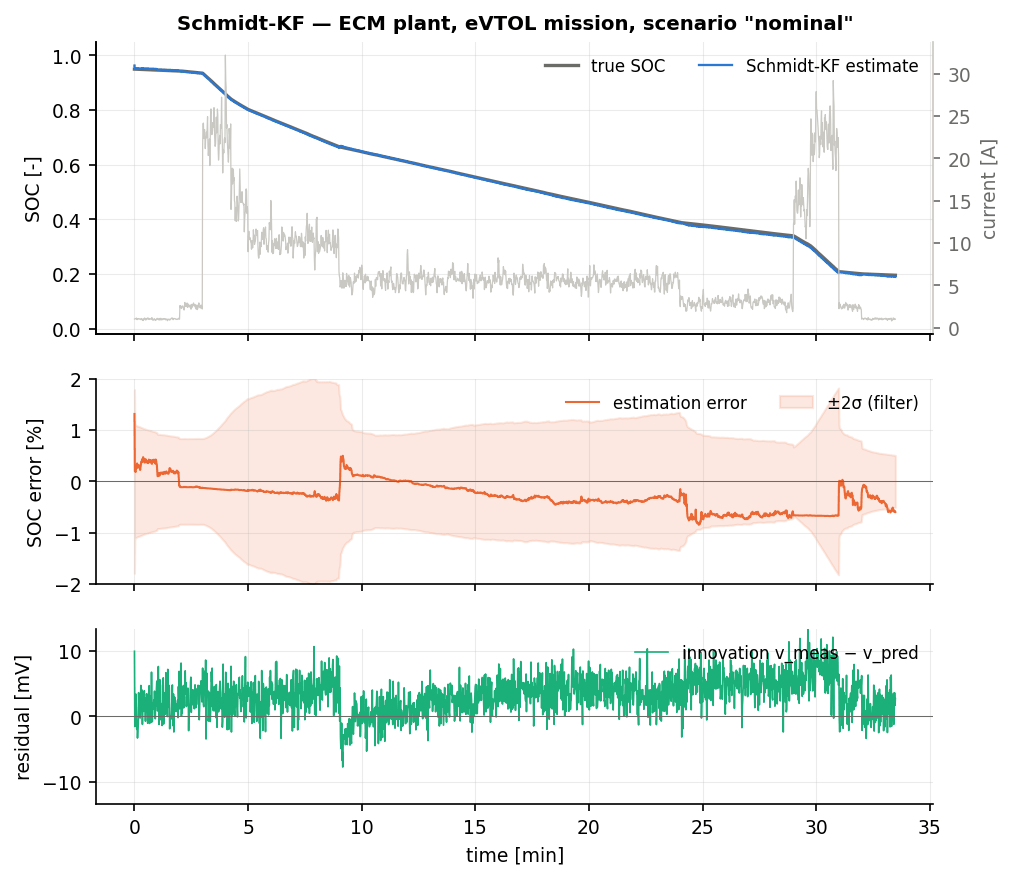
\includegraphics[width=\textwidth]{figures/cell_SchmidtKF_nominal.png}
\caption{Schmidt-KF on the nominal eVTOL mission: true and estimated SOC (top), estimation error
with the $\pm2\sigma$ band (middle), voltage residual (bottom).  The $2\sigma$ band is visibly
wider than the EKF's and modulated by the current profile, which is the consider contribution
$\mH^c\mP_{cc}(\mH^c)^\T$ at work.}
\end{figure}
\begin{figure}[H]\centering
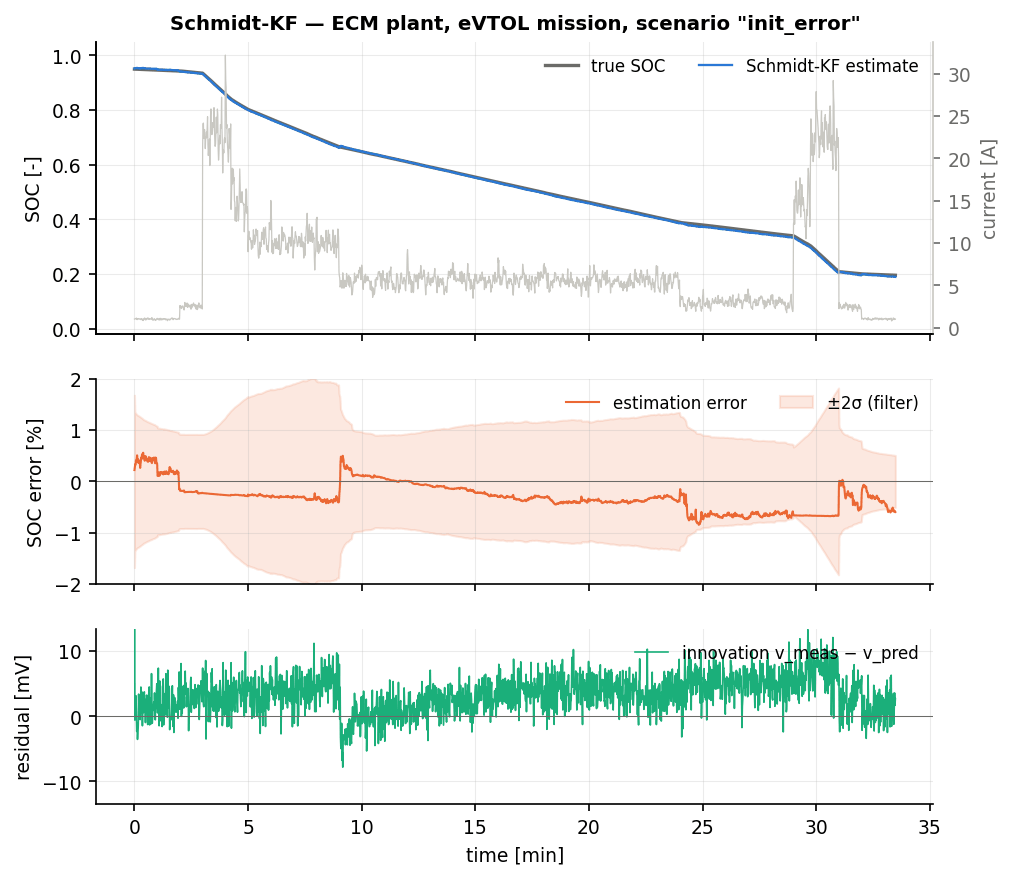
\includegraphics[width=\textwidth]{figures/cell_SchmidtKF_init_error.png}
\caption{Schmidt-KF with a 35\,\% initial SOC error.}
\end{figure}
\begin{figure}[H]\centering
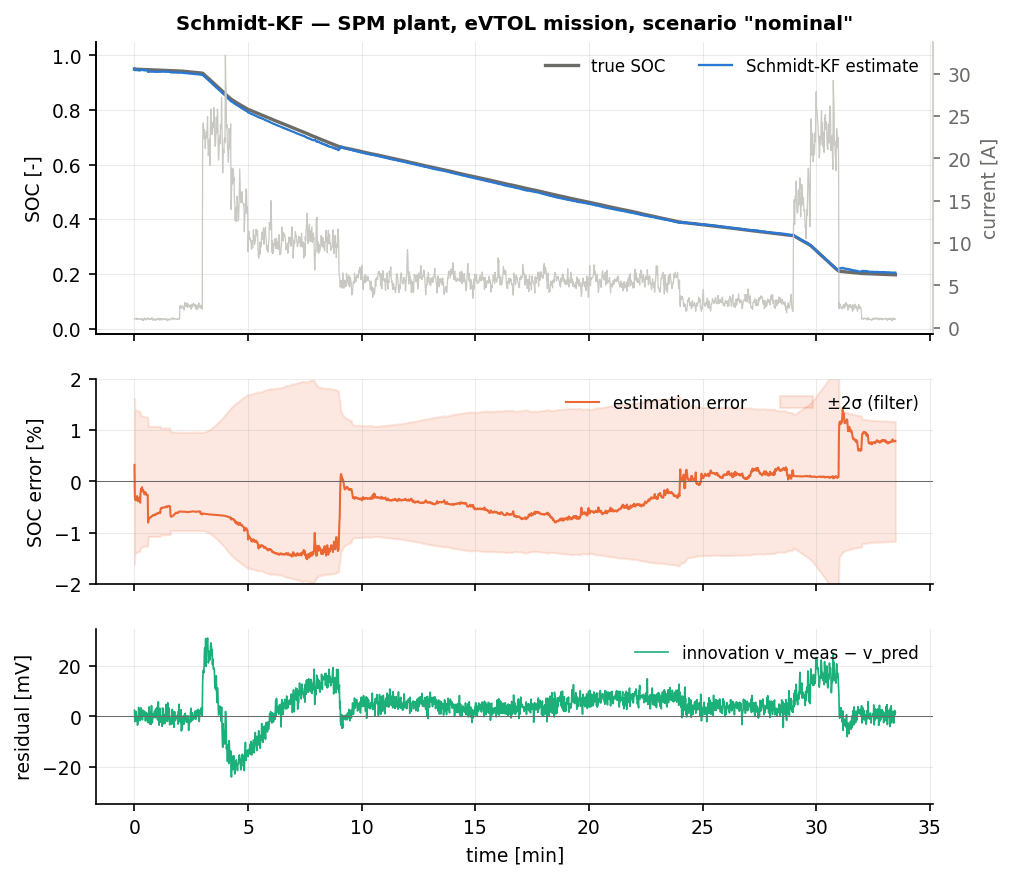
\includegraphics[width=\textwidth]{figures/cellspm_SchmidtKF_nominal.png}
\caption{SchmidtKF on the SPM (electrochemical) plant, nominal eVTOL mission.  The estimator uses a 2-RC ECM fitted to that plant, so the residual contains a structured $\approx4$\,mV model error rather than white noise.}
\end{figure}

All numbers below are 3-seed means from the final run, in \% SOC
(\texttt{rmse}/\texttt{rmse\_ss}); the EKF column is the plain EKF on the same data.

\paragraph{ECM plant, eVTOL mission.}
The Schmidt-KF behaves exactly as the theory predicts: it pays a modest price where the model is
right and wins decisively where it is wrong.
\begin{center}\small
\begin{tabular}{@{}lccl@{}}
\toprule
Scenario & Schmidt-KF & EKF & Comment\\
\midrule
\texttt{nominal}        & $0.38/0.46$ & $0.15/0.05$ & $9\times$ worse (ss) --- the price of the low gain\\
\texttt{init\_error}    & $0.43/0.46$ & $0.14/0.05$ & converges at $t=0$\,s\\
\texttt{cold}           & $1.42/1.54$ & $0.20/0.16$ & worst case: $\alpha_{R_0}=2.1$ quadruples the inflation\\
\texttt{noise\_step}    & $0.87/1.14$ & $0.18/0.12$ & already de-weighted, cannot de-weight more\\
\texttt{hot}            & $0.23/0.21$ & $0.20/0.03$ & ---\\
\texttt{aged\_cell}     & $\mathbf{0.71/0.59}$ & $1.18/1.52$ & $\mathbf{2.6\times}$ better (ss)\\
\texttt{param\_mismatch}& $\mathbf{0.51/0.45}$ & $1.28/1.36$ & $\mathbf{3.0\times}$ better\\
\texttt{combined}       & $\mathbf{5.20/1.09}$ & $16.02/12.44$ & $\mathbf{11\times}$ better (ss); converges at 1038\,s\\
\texttt{current\_bias}  & $\mathbf{0.33/0.33}$ & $0.54/0.61$ & $1.8\times$ better\\
\texttt{sensor\_dropout}& $0.38/0.46$ & $0.72/0.46$ & rmse $1.9\times$ better, steady state tied\\
\texttt{preisach}       & $1.02/0.55$ & $0.58/0.20$ & $2.8\times$ \emph{worse} --- see below\\
\texttt{outliers}       & $0.77/0.83$ & $0.52/0.21$ & no outlier mechanism; see Ch.~\ref{ch:huberekf}\\
\bottomrule
\end{tabular}
\end{center}
Acceptance is met everywhere: \texttt{nominal} $\texttt{rmse\_ss}=0.46\,\%<2\,\%$,
\texttt{init\_error} $t_\mathrm{conv}=0$\,s, no divergence in any of the twelve ECM or nine SPM
scenarios, and the worst steady-state error over all ECM scenarios is $1.54\,\%$ (\texttt{cold}),
still inside the acceptance band.

The two headline numbers are \texttt{param\_mismatch} and \texttt{combined}.  In
\texttt{param\_mismatch} the estimator is given $R_0$ that is $30\,\%$ too small; the EKF converts
the resulting current-proportional voltage bias into a persistent SOC bias of $1.36\,\%$, whereas
the consider filter --- which was told that $R_0$ might be wrong by $20\,\%$ --- discounts exactly
that residual and ends at $0.45\,\%$.  In \texttt{combined} the failure of the EKF is spectacular:
the ageing law makes the true $R_0$ $25\,\%$ larger than the estimator's, and at
0\,\ensuremath{{}^\circ}C the Arrhenius factor multiplies that error by $2.1$, so during the
32\,A take-off hover the predicted voltage is 200\,mV too high.  The EKF reads this as a collapse
of the SOC, never converges ($t_\mathrm{conv}=$ ``--'', $\texttt{rmse\_ss}=12.44\,\%$), while the
Schmidt-KF's innovation covariance is inflated by three orders of magnitude during exactly those
seconds: it converges at $t=1038$\,s and finishes at $1.09\,\%$.

\paragraph{Where it costs.}  On \texttt{nominal} the filter is nine times less accurate than the
EKF in steady state, because a gain that is $40$--$660$ times smaller cannot reject the process
noise as well.  On \texttt{cold} the same mechanism goes too far: the consider term is proportional
to $\alpha_{R_0}(T)^2$, so a sensible $20\,\%$ relative uncertainty at 25\,\ensuremath{{}^\circ}C
becomes a very heavy de-weighting at $-10$\,\ensuremath{{}^\circ}C and the steady-state error
rises to $1.54\,\%$.  A practical BMS would make $\rho_{R_0}$ temperature dependent (the Arrhenius
activation energy is the uncertain quantity, not the room-temperature value); a single-seed sweep
gives \texttt{cold} $1.16\,\%$ and \texttt{param\_mismatch} $0.48\,\%$ at $\rho_{R_0}=10\,\%$
against $1.70\,\%$ and $0.38\,\%$ at $\rho_{R_0}=20\,\%$, so the 5\,\%/20\,\% pair was kept because
it is the literature-standard statement of a cell tolerance, not because it is optimal here.

\paragraph{Preisach.}  With the corrected sign convention of the final plant (charging branch above
the discharging branch) the \texttt{preisach} scenario is now a case the Schmidt-KF loses:
$0.55\,\%$ against the EKF's $0.20\,\%$, and it converges at 21\,s rather than 16\,s.  The reason is
the same low gain that helps elsewhere.  The Preisach residual is a \emph{hysteresis} error --- it
is uncorrelated with the current magnitude and therefore falls entirely outside the
$\mH^c\mP_{cc}(\mH^c)^\T$ term, which only inflates $\mS$ in proportion to $i^2$.  The filter
consequently de-weights the measurement without gaining any protection against this particular
error, and simply tracks more slowly.  This is worth stating plainly: a consider filter protects
against the parameters it is told about and against nothing else.

\paragraph{SPM (electrochemical) plant.}  On the SPM rows the estimators run a 2-RC ECM fitted to a
single-particle model with Butler--Volmer kinetics and $\tau_2=556$\,s, leaving a structured
$\approx4$\,mV residual instead of white noise.  This is the Schmidt-KF's best result in the whole
benchmark: $0.69/0.51\,\%$ on \texttt{nominal} against the EKF's $3.65/3.73\,\%$, a factor of
$7.3$, and it is the best of the eight filters in this family on seven of the nine SPM scenarios
(\texttt{sensor\_dropout} $0.69/0.50\,\%$ vs.\ $5.13/5.31\,\%$, $10.6\times$;
\texttt{current\_bias} $1.02/0.71\,\%$ vs.\ $4.93/5.69\,\%$, $8.0\times$; \texttt{hot}
$0.43/0.44\,\%$ vs.\ $2.08/2.16\,\%$; \texttt{param\_mismatch} $1.10/0.75\,\%$ vs.\
$2.87/3.13\,\%$; \texttt{cold} $2.49/2.44\,\%$ vs.\ $7.07/7.35\,\%$).  The mechanism is worth
spelling out because it is the whole point of the method.  The 4\,mV SPM residual is dominated by
the concentration overpotential, which is a slow, current-driven function --- precisely the shape
of $\partial v/\partial R_0 \cdot \delta R_0 = -i\,\delta R_0$ and of the slow-branch voltage.  A
plain EKF has no model for it and therefore attributes it to the only slow state it has, the SOC,
which is why every unprotected filter sits at $3.1$--$4.1\,\%$.  The consider covariance inflates
$\mS$ by exactly $i^2\sigma_{R_0}^2\alpha_{R_0}^2$, which is the right shape and the right order of
magnitude, so the SOC channel simply stops listening while the current is large and the
$(\soc,v_2)$ ambiguity never gets a chance to absorb the model error.  The only cost is on the
transient: \texttt{init\_error} takes 360\,s to converge (EKF: immediately, but to the wrong value)
and \texttt{cold} 939\,s.  The generic lesson is that a consider filter is the right tool when the
unmodelled physics has the \emph{same signature} as one of the consider parameters --- which for an
electrochemical cell described by an equivalent circuit is usually the case.

\paragraph{Consistency.}  Finally, the point of the method is consistency, not RMSE.  On
\texttt{param\_mismatch} the EKF's reported $2\sigma$ SOC band is $\pm0.2\,\%$ while its actual
error is $1.36\,\%$ --- wrong by seven standard deviations and unaware of it.  The Schmidt-KF's band
grows with the accumulated ampere-hours through \eqref{eq:sk-tuxx} and with the current through
\eqref{eq:sk-S}, and covers its own error.  For a flight-critical remaining-energy computation that
difference matters more than a factor of three in RMSE.

\section{Summary}
Use the Schmidt--Kalman filter when the model parameters are uncertain but the mission does not
excite them enough to identify them safely --- which is the normal situation for capacity and
resistance during a single eVTOL flight.  It costs about 2.7 times an EKF step (and 4\,kB more RAM, most of it a second copy of the
model), never destabilises, and turns a silent bias into an honest covariance; on the
parameter-error scenarios of this benchmark it is also three to eleven times more accurate, and on
the electrochemical plant --- where the unmodelled physics has the same current-driven signature as
the consider parameters --- it is seven times more accurate than the EKF and the best filter of the
family.  Do not use it when the data
\emph{do} identify the parameters (a full charge--discharge cycle, a rest period): a joint or dual
filter will then be strictly better, because the consider filter throws that information away by
construction.  Do not use it as an outlier defence either --- it de-weights the measurement by a
fixed, current-dependent amount, not by how surprising the measurement is.
